\chapter{Lagrangian, các trường và các quá trình hạt cục bộ}

Các trường boson, các trường fermion và trường điện từ đều tuân theo những phương trình kiểu sóng. Các phương trình ấy chứa chính các trường cùng với các đạo hàm theo không gian và thời gian của chúng. Người ta có thể viết riêng một phương trình chuyển động cho từng trường, nhưng một Lagrangian gom toàn bộ hệ vào một biểu thức cô đọng duy nhất. Áp dụng quy tắc Euler--Lagrange cho biểu thức đó sẽ cho ra các phương trình của mọi trường cùng một lúc.

Cách xây dựng này liên hệ chặt chẽ với nguyên lý tác dụng dừng. Ở đây, nhiệm vụ trước mắt cụ thể hơn: xác định một Lagrangian trường phụ thuộc vào những gì, dùng nó để thu được một vài phương trình cổ điển, rồi sau đó diễn giải lại chính các biểu thức trường ấy theo cơ học lượng tử. Trong lý thuyết lượng tử, Lagrangian chi phối chuyển động và tương tác của hạt, và rốt cuộc là các biên độ cũng như tiết diện của va chạm.

\section{Mã gọn cho các phương trình trường}

Đối với một trường vô hướng, mật độ Lagrangian phụ thuộc vào trường và các đạo hàm bậc nhất của nó,
\begin{equation}
\mathcal L
=
\mathcal L\!\left(\phi,\partial_t\phi,\partial_x\phi,\ldots\right)
=
\mathcal L\!\left(\phi,\partial_\mu\phi\right).
\end{equation}
Danh sách tường minh các đạo hàm theo thời gian và theo không gian thường hữu ích hơn khi tính toán; ký hiệu \(\partial_\mu\phi\) viết gọn chính danh sách đó dưới dạng tương đối tính.

\begin{figure}[htbp]
\centering
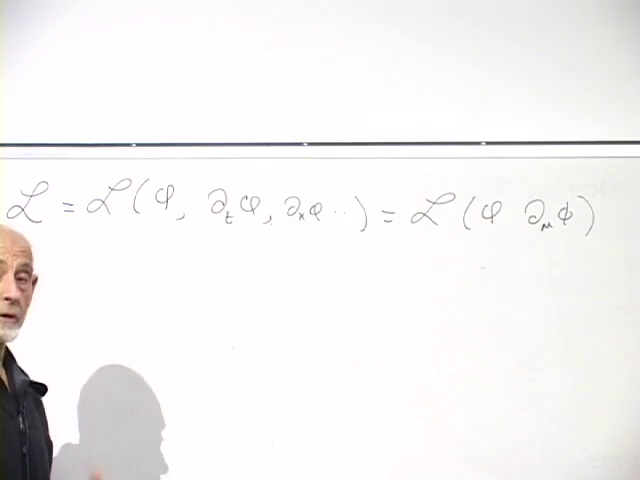
\includegraphics[width=0.82\textwidth]{lecture_09_figure_03.png}
\caption{Sự phụ thuộc của một Lagrangian trường vô hướng vào trường và các đạo hàm không-thời gian của nó.}
\lectureframe{00:03:56}
\end{figure}

Phương trình Euler--Lagrange cho trường là
\begin{equation}
\frac{\partial}{\partial t}
\frac{\partial\mathcal L}{\partial\dot\phi}
+
\frac{\partial}{\partial x}
\frac{\partial\mathcal L}{\partial\phi_x}
+
\frac{\partial}{\partial y}
\frac{\partial\mathcal L}{\partial\phi_y}
+
\frac{\partial}{\partial z}
\frac{\partial\mathcal L}{\partial\phi_z}
=
\frac{\partial\mathcal L}{\partial\phi},
\end{equation}
trong đó
\begin{equation}
\dot\phi=\frac{\partial\phi}{\partial t},
\qquad
\phi_x=\frac{\partial\phi}{\partial x},
\qquad
\phi_y=\frac{\partial\phi}{\partial y},
\qquad
\phi_z=\frac{\partial\phi}{\partial z}.
\end{equation}
Nếu \(\mathcal L\) chứa nhiều trường, thì quy tắc này được áp dụng một lần cho mỗi trường. Kết quả là hệ các phương trình chuyển động.

Ví dụ vô hướng đơn giản nhất là
\begin{equation}
\begin{split}
\mathcal L
&=
\frac12\dot\phi^2
-\frac12\phi_x^2
-\frac12\phi_y^2
-\frac12\phi_z^2
-V(\phi)
\\
&=
\frac12\dot\phi^2-\frac12(\boldsymbol\nabla\phi)^2-V(\phi).
\end{split}
\end{equation}
Các hạng đạo hàm không gian mang dấu ngược với hạng đạo hàm theo thời gian. Lấy đạo hàm từng hạng cho
\begin{align}
\frac{\partial\mathcal L}{\partial\dot\phi}&=\dot\phi,
&
\frac{\partial\mathcal L}{\partial\phi_i}&=-\phi_i,
&
\frac{\partial\mathcal L}{\partial\phi}&=-V'(\phi),
\end{align}
và do đó
\begin{equation}
\ddot\phi-\nabla^2\phi=-V'(\phi).
\end{equation}

\begin{figure}[htbp]
\centering
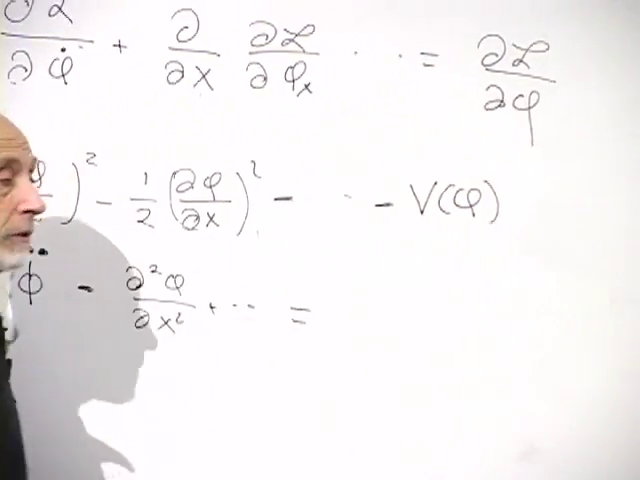
\includegraphics[width=0.74\textwidth]{lecture_09_figure_04.png}
\caption{Phương trình Euler--Lagrange, Lagrangian trường vô hướng và phương trình trường do \(V(\phi)\) sinh ra.}
\lectureframe{00:08:23}
\end{figure}

Đây là phương trình do Lagrangian vô hướng sinh ra.\editorialnote{Khung hình được giữ lại bị cắt ở mép trái; phần hoàn chỉnh được hiển thị được xác định từ phép suy dẫn bằng lời ngay xung quanh.}

Ở đây \(V(\phi)\) là mật độ thế năng của trường. Một đóng góp hằng vào \(V\) không ảnh hưởng gì đến phương trình này vì đạo hàm của nó triệt tiêu. Một thế tuyến tính là khả dĩ về mặt đại số, nhưng nó không có cận dưới: năng lượng của trường có thể chạy xuống âm vô cùng. Vì vậy, ví dụ ổn định đầu tiên là
\begin{equation}
V(\phi)=\frac12m^2\phi^2,
\qquad
V'(\phi)=m^2\phi,
\end{equation}
từ đó cho
\begin{equation}
\ddot\phi-\nabla^2\phi=-m^2\phi.
\end{equation}

Để làm rõ ý nghĩa của \(m\), hãy thế một sóng phẳng,
\begin{equation}
\phi(\mathbf x,t)=\phi_0e^{i\omega t-i\mathbf k\cdot\mathbf x}.
\end{equation}
Khi đó
\begin{equation}
\ddot\phi=-\omega^2\phi,
\qquad
\nabla^2\phi=-\mathbf k^2\phi,
\end{equation}
nên phương trình sóng trở thành
\begin{equation}
-\omega^2\phi+\mathbf k^2\phi=-m^2\phi.
\end{equation}
Sau khi khử \(\phi\),
\begin{equation}
\omega^2=\mathbf k^2+m^2.
\end{equation}
Trong hệ đơn vị \(\hbar=c=1\), tần số là năng lượng và số sóng là xung lượng. Do đó
\begin{equation}
E^2=\mathbf p^2+m^2,
\end{equation}
hoặc, khi khôi phục các lũy thừa của \(c\), \(E^2=\mathbf p^2c^2+m^2c^4\). Tham số \(m\) là khối lượng của một lượng tử của trường.

Tính bất biến tương đối tính có thể được áp đặt ngay ở mức biểu thức gọn. Nếu \(\mathcal L\) là một vô hướng Lorentz, thì các phương trình chuyển động của nó là bất biến Lorentz. Dấu tương đối giữa các đạo hàm theo thời gian và theo không gian chính là dấu không-thời gian quen thuộc của thuyết tương đối hẹp.

\section{Tính phi tuyến và các trường cổ điển ghép cặp}

Các lũy thừa cao hơn của trường đưa vào một kiểu hành vi mới. Nếu
\begin{equation}
V(\phi)=\frac12m^2\phi^2+g\phi^3,
\end{equation}
thì
\begin{equation}
\ddot\phi-\nabla^2\phi=-m^2\phi-3g\phi^2.
\end{equation}
Các hạng bậc hai trong Lagrangian cho những phương trình tuyến tính theo trường. Các hạng bậc ba và cao hơn cho những phương trình phi tuyến.

Sự phân biệt ấy thấy rõ trong chuyển động của các gói sóng. Với một phương trình tuyến tính, có thể cộng một gói truyền sang phải với một gói truyền sang trái để được một nghiệm khác. Chúng chồng lấp và giao thoa với nhau trong một lúc, rồi đi xuyên qua nhau và xuất hiện trở lại với hình dạng ban đầu. Khi có các hạng phi tuyến, các gói ảnh hưởng lẫn nhau. Chúng có thể tán xạ, biến dạng hoặc vỡ thành những sóng phức tạp hơn. Sự giao thoa tạm thời của sóng tuyến tính không phải là tương tác; một biến đổi kéo dài trong các gói là dấu hiệu của tính phi tuyến.

Mẫu hình ấy cũng xuất hiện với hai trường vô hướng. Hãy đặt
\begin{align}
\mathcal L
&=
\frac12(\partial_\mu\phi)(\partial^\mu\phi)
+\frac12(\partial_\mu\rho)(\partial^\mu\rho)
-V(\phi,\rho),
\\
V(\phi,\rho)
&=
\frac12m^2\phi^2+\frac12M^2\rho^2+\rho\phi^2.
\end{align}
Không có hạng cuối, hai phương trình là độc lập,
\begin{equation}
\ddot\phi-\nabla^2\phi=-m^2\phi,
\qquad
\ddot\rho-\nabla^2\rho=-M^2\rho.
\end{equation}
Chúng mô tả các lượng tử của hai loại, với khối lượng \(m\) và \(M\). Khi đưa thêm hạng trộn vào,
\begin{align}
\ddot\phi-\nabla^2\phi&=-m^2\phi-2\rho\phi,
\\
\ddot\rho-\nabla^2\rho&=-M^2\rho-\phi^2.
\end{align}
Mỗi phương trình giờ đây đều chứa trường kia. Các phương trình vừa ghép cặp vừa phi tuyến: một gói \(\phi\) tán xạ một gói \(\rho\), và ngược lại. Các hạng đạo hàm chi phối hệ thức năng lượng--xung lượng, các hạng bậc hai không đạo hàm xác định khối lượng, còn hạng trộn bậc cao hơn mã hóa tương tác. Đây là khuôn mẫu cổ điển cơ bản.

\section{Trường Dirac và một ghép vô hướng}

Đối với một trường Dirac, phương trình là bậc nhất theo thời gian. Dưới dạng viết tắt một chiều, với việc mở rộng sang ba phương không gian đã được ngầm hiểu, cấu trúc các hạng của nó là
\begin{equation}
i\dot\Psi
\simeq
i\alpha\frac{\partial\Psi}{\partial x}+m\beta\Psi,
\qquad
i\boldsymbol\alpha\cdot\boldsymbol\nabla\Psi
=i\sum_i\alpha_i\frac{\partial\Psi}{\partial x_i}.
\end{equation}
Các ma trận \(\alpha_i\) và \(\beta\) tác dụng lên các thành phần của \(\Psi\). Một Lagrangian tương ứng chứa một hạng tuyến tính theo \(\partial_t\Psi\), một song tuyến tính đạo hàm không gian có chứa \(\alpha_i\), và song tuyến tính khối lượng \(m\Psi^\dagger\beta\Psi\). Ở đây chỉ cần sự kiện về cấu trúc đó.\editorialnote{Dấu, ngoặc và vị trí đặt của \(i\) trong Lagrangian Dirac được thử viết ra được nguồn để ngỏ một cách tường minh. Từ đó không suy ra công thức chính xác nào phụ thuộc quy ước.}

\begin{figure}[htbp]
\centering
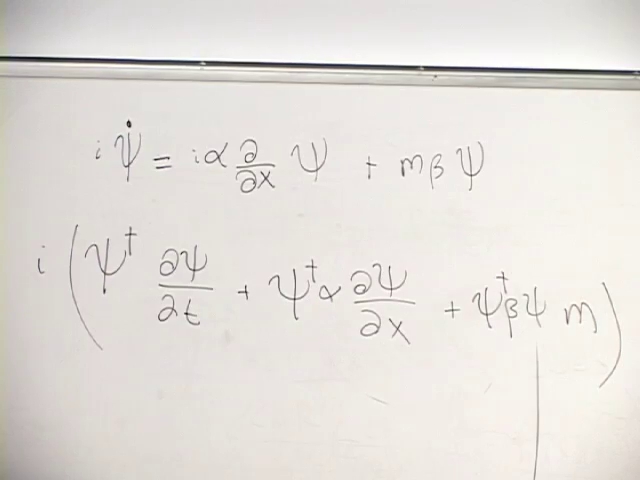
\includegraphics[width=0.76\textwidth]{lecture_09_figure_05.png}
\caption{Các hạng đạo hàm theo thời gian, đạo hàm theo không gian và khối lượng trong phần thảo luận về trường Dirac.}
\lectureframe{00:25:37}
\end{figure}

\begin{classroomqa}
\lecturetimestamp{00:26:37}
\audiencequestion{Dấu ngoặc trong Lagrangian Dirac thử viết ra có được đặt đúng không, với \(i\) nhân toàn bộ biểu thức?}
\lecturerresponse{Vị trí đặt ấy không được chốt ở đây một cách chắc chắn, và điều đó không cần cho ý chính về mặt cấu trúc: tồn tại một Lagrangian sinh ra phương trình Dirac.}
\end{classroomqa}

Bây giờ thêm một trường vô hướng \(\phi\). Tích ngây thơ \(\Psi^\dagger\Psi\,\phi\) không phải là một vô hướng Lorentz. Chèn cùng ma trận Dirac xuất hiện trong hạng khối lượng vào, ta được
\begin{equation}
\mathcal L_{\mathrm{int}}
\propto
\Psi^\dagger\beta\Psi\,\phi.
\end{equation}
Tương đương, \(\Psi^\dagger\beta\Psi\) là song tuyến tính Dirac vô hướng. Lấy biến phân của Lagrangian đầy đủ sẽ thêm một hạng tỉ lệ với \(\phi\) vào phương trình Dirac và một nguồn tỉ lệ với \(\Psi^\dagger\beta\Psi\) vào phương trình vô hướng. Hai trường tán xạ lẫn nhau.

\begin{classroomqa}
\lecturetimestamp{00:28:03}
\audiencequestion{Ma trận \(\beta\) được chèn vào tương tác vô hướng--fermion có phải chính là \(\beta\) xuất hiện trong hạng khối lượng Dirac không?}
\lecturerresponse{Đúng. Đó là cùng một ma trận Dirac.}
\end{classroomqa}

Phép so sánh
\begin{equation}
m\Psi^\dagger\beta\Psi
\qquad\hbox{and}\qquad
\Psi^\dagger\beta\Psi\,\phi
\end{equation}
khiến ghép đó trông như một tham số khối lượng được thay bằng một trường vô hướng. Nhận xét này sẽ quay lại khi ta xét một trường có giá trị chân không khác không ở gần cuối.

Cho đến đây, cách diễn giải vẫn là cổ điển: các gói sóng tán xạ những gói sóng khác. Cùng phép đại số ấy có một ý nghĩa hạt sắc nét hơn khi các trường trở thành toán tử.

\section{Các lũy thừa của trường lượng tử làm gì}

Một trường lượng tử vô hướng thực chứa cả toán tử tạo lẫn toán tử hủy. Về sơ đồ,
\begin{equation}
\phi(x)\sim A^+(x)+A^-(x),
\end{equation}
trong đó \(A^+\) tạo ra một lượng tử còn \(A^-\) hủy một lượng tử. Do đó, \(\phi^3(x)\) chứa bốn kiểu quá trình cục bộ:
\begin{equation}
\phi^3
\sim
(A^+)^3+(A^+)^2A^-+A^+(A^-)^2+(A^-)^3,
\end{equation}
trong đó các chi tiết về thứ tự và các hệ số số học được lược bỏ trong cách đọc sơ đồ này. Bốn sự thay đổi số hạt là
\begin{equation}
3\longrightarrow0,
\qquad
0\longrightarrow3,
\qquad
2\longrightarrow1,
\qquad
1\longrightarrow2.
\end{equation}
Ba thừa số trường đều tác dụng tại cùng một điểm \(x\). Vì thế một hạng bậc ba đơn lẻ bao gồm sự hủy ba hạt, sự tạo ba hạt, sự hợp nhất của hai lượng tử thành một, và sự phân rã của một lượng tử thành hai. Trong một biên độ vật lý, về sau một số cách đọc cục bộ này có thể bị loại bởi bảo toàn năng lượng--xung lượng, nhưng tất cả chúng đều có mặt ngay trong chính tích toán tử.

Các hạng tự do bậc hai có vai trò khác. Trước hết hãy tạm bỏ qua hệ số chuẩn hóa của hiệu giữa hai điểm lân cận \(x\) và \(x'\):
\begin{equation}
\partial_x\phi
\ \propto\
\phi(x)-\phi(x').
\end{equation}
Bình phương rồi khai triển cho cấu trúc hạng
\begin{align}
\frac12(\partial_x\phi)^2
&\ \propto\
\frac12\bigl[\phi(x)-\phi(x')\bigr]^2
\\
&=
\frac12\phi(x)^2
+\frac12\phi(x')^2
-\phi(x)\phi(x').
\end{align}
Mỗi bình phương tại cùng một điểm có vài cách đọc theo toán tử: nó có thể tạo hai lượng tử, hủy hai lượng tử, hoặc hủy rồi tái tạo một lượng tử ngay tại điểm đó. Các hạng ấy không vận chuyển một hạt. Hạng chéo có thể hủy một lượng tử tại \(x'\) và tạo nó tại \(x\), hoặc ngược lại. Vì vậy nó hoạt động như một hạng nhảy giữa các láng giềng gần nhất. Các thừa số lặp lại mang một hạt từ \(x\) sang \(x'\), rồi sang \(x''\), và tiếp tục như thế. Các hạng đạo hàm bậc hai chi phối sự lan truyền tự do; các hạng bậc ba và cao hơn thì tán xạ, tạo và hủy hạt.

\begin{classroomqa}
\lecturetimestamp{00:36:07}
\audiencequestion{Biểu diễn sai phân hữu hạn của đạo hàm có nên bao gồm độ tách \(x-x'\) không?}
\lecturerresponse{Có. Nếu gọi độ tách đó là \(L\) thì sau khi bình phương hiệu, ta có thêm thừa số \(L^{-2}\). Thừa số số học ấy làm thay đổi hệ số nhưng không làm đổi cách diễn giải theo bước nhảy.}
\end{classroomqa}

Khôi phục độ tách vào thì được
\begin{align}
\frac12(\partial_x\phi)^2
&\longrightarrow
\frac{1}{2L^2}\bigl[\phi(x)-\phi(x')\bigr]^2
\\
&=
\frac{1}{2L^2}\phi(x)^2
+\frac{1}{2L^2}\phi(x')^2
-\frac{1}{L^2}\phi(x)\phi(x').
\end{align}

Hạng khối lượng cũng là bậc hai nhưng không chứa đạo hàm:
\begin{equation}
\frac12m^2\phi(x)^2.
\end{equation}
Cách đọc một-hạt của nó là một lượng tử tới bị hấp thụ và phát lại tại cùng một điểm. Nó không làm lượng tử chuyển chỗ; nó gán trọng số, hay theo nghĩa đó là đếm, sự hiện diện của nó ở đó. Cùng bình phương toán tử ấy cũng chứa các cách đọc tạo hai hạt và hủy hai hạt của nó. Vì vậy, sự khác biệt có liên quan đến chuyển động là giữa một hạng chéo nối các điểm lân cận và một chèn khối lượng tác dụng trong một điểm.

\section{Đỉnh cục bộ của điện động lực học lượng tử}

Những phác họa sơ cấp về quá trình hạt này là khởi đầu của các biểu đồ Feynman. Ví dụ trung tâm là điện động lực học lượng tử, lý thuyết của electron, positron và photon.

Phương trình Dirac có các mode năng lượng dương và năng lượng âm. Theo ngôn ngữ cũ, \(\Psi\) chứa các toán tử hủy cho cả hai loại mode, còn \(\Psi^\dagger\) chứa các toán tử tạo tương ứng. Việc lấy đi một electron năng lượng âm được diễn giải lại thành việc tạo ra một positron năng lượng dương. Sau phép đổi nhãn đó, phân tích sơ đồ hữu ích là
\begin{align}
\Psi
&\sim
C^-_{e^-}+C^+_{e^+},
\\
\Psi^\dagger
&\sim
C^+_{e^-}+C^-_{e^+}.
\end{align}
Vì vậy \(\Psi\) hủy một electron hoặc tạo một positron, còn \(\Psi^\dagger\) tạo một electron hoặc hủy một positron. Trong lối viết tắt này không hàm ý chuẩn hóa, nhãn spin hay tích phân theo xung lượng nào.

Tương tác QED ghép dòng Dirac với thế vectơ điện từ. Trong ký hiệu theo thành phần được dùng ở đây, cấu trúc của nó là
\begin{equation}
\mathcal L_{\mathrm{QED,int}}
\sim
e\left(
\Psi^\dagger\Psi\,A_0
+
\Psi^\dagger\boldsymbol{\alpha}\Psi\mathbin{\boldsymbol{\cdot}}\mathbf A
\right),
\end{equation}
trong đó
\begin{equation}
J^0=\Psi^\dagger\Psi,
\qquad
\mathbf J=\Psi^\dagger\boldsymbol{\alpha}\Psi.
\end{equation}
Ký hiệu \(\sim\) là quan trọng: dấu tương đối giữa hạng thời gian và hạng không gian phụ thuộc vào quy ước metric và quy ước thế vectơ. Phát biểu bất biến là dòng bốn được co với thế bốn.\editorialnote{Nguồn cố định các thành phần thời gian và không gian của dòng nhưng không chốt một quy ước metric cho phép co theo thành phần.}

Trường photon \(A_\mu\) tự thân cũng chứa các toán tử tạo và hủy photon. Tính vectơ của nó còn mang theo phân cực của photon---một ``lá cờ'' chỉ hướng nhỏ bên cạnh xung lượng của nó.

\begin{classroomqa}
\lecturetimestamp{00:44:28}
\audiencequestion{Làm sao tương tác lại có thể là vô hướng khi \(A_\mu\) là một vectơ còn thoạt đầu thừa số fermion dường như là một vô hướng?}
\lecturerresponse{Các fermion cũng cung cấp một vectơ bốn: \(\Psi^\dagger\Psi\) là thành phần thời gian của nó còn \(\Psi^\dagger\boldsymbol\alpha\Psi\) là thành phần không gian. Co dòng đó với \(A_\mu\) sẽ cho một vô hướng.}
\end{classroomqa}

Nhân các nội dung toán tử của \(\Psi^\dagger\), \(\Psi\) và \(A_\mu\) cho ta bốn cách đọc quen thuộc của một đỉnh cục bộ:
\begin{enumerate}
\item một electron phát ra một photon;
\item một electron hấp thụ một photon;
\item một electron và một positron hủy nhau thành một photon;
\item một photon tạo ra một cặp electron--positron.
\end{enumerate}
Đối với cách đọc thứ nhất, \(\Psi\) hủy electron đi vào, \(\Psi^\dagger\) tạo electron đi ra, và trường photon tạo ra photon. Chọn phần hủy photon thì được sự hấp thụ. Chọn các phần của positron thì được hủy cặp hoặc tạo cặp. Một hạng cục bộ chứa toàn bộ họ quá trình đó.

Trong một sơ đồ dòng fermion, mũi tên trên một đường positron chỉ ngược với hướng truyền của positron. Với quy ước đó, mũi tên fermion đi liên tục qua mọi đỉnh QED được phép. Bốn cách đọc khác nhau ở chỗ chuyển các chân ngoài giữa phía đi vào và phía đi ra, chứ không phải ở chỗ bẻ gãy đường dòng fermion.

Mỗi cách đọc này đều mang cùng một hệ số \(e\), tức điện tích trong quy ước vi mô đang được dùng. Hệ số này là điện tích \(e\), không phải hằng số cấu trúc tinh tế, mặc dù hai đại lượng liên hệ chặt chẽ. Biên độ của đỉnh tỉ lệ với \(e\); sau khi kể hết các thừa số động học và chuẩn hóa, thang xác suất tương ứng tỉ lệ với \(e^2\).

\begin{classroomqa}
\lecturetimestamp{00:49:44}
\audiencequestion{Cách đọc từ photon sang electron--positron có cùng hệ số như các cách đọc khác của đỉnh không?}
\lecturerresponse{Có. Nó mang cùng hệ số điện tích \(e\).}
\end{classroomqa}

\begin{classroomqa}
\lecturetimestamp{00:49:59}
\audiencequestion{Có nhất thiết phải có một hệ số tỉ lệ, vì xác suất không có đơn vị không?}
\lecturerresponse{Trong quy ước vi mô tự nhiên đang được dùng, điện tích \(e\) là vô thứ nguyên. Nó đặt thang biên độ, còn bình phương của nó cung cấp thang xác suất.}
\end{classroomqa}

Một hình dung cụ thể là một electron đập vào một bức tường rồi dừng lại đột ngột. Có một xác suất nào đó để năng lượng và động lượng rời đi dưới dạng một photon. Thừa số điện từ sơ cấp trong biên độ bức xạ đó là \(e\), nên thang xác suất của nó chứa \(e^2\). Phát biểu này tách riêng thừa số ghép; xác suất thực tế còn phụ thuộc vào trạng thái của electron và vào động học.

\begin{figure}[htbp]
\centering
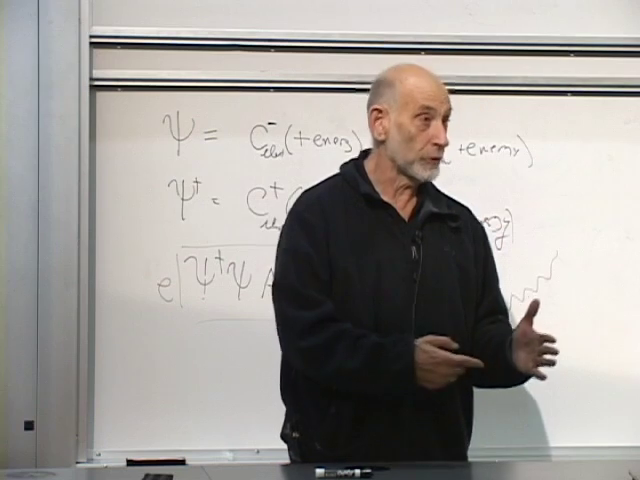
\includegraphics[width=0.78\textwidth]{lecture_09_figure_06.png}
\caption{Thành phần toán tử electron và positron của \(\Psi\) và \(\Psi^\dagger\), kèm một phác họa tương tác electron--photon.}
\lectureframe{00:50:39}
\end{figure}

\begin{classroomqa}
\lecturetimestamp{00:51:15}
\audiencequestion{Điện tích có đơn vị không?}
\lecturerresponse{Không, trong quy ước vi mô tự nhiên được dùng ở đây thì không. Điện tích vĩ mô thường được báo bằng coulomb, nhưng lý thuyết hạt đo điện tích tương đối với một đơn vị cơ bản được chọn. Trong đơn vị Planck hoặc các đơn vị tự nhiên khác, các đại lượng được biểu diễn bằng những số thuần túy.}
\end{classroomqa}

Sự tương phản này là về quy ước và thang đo. Coulomb thuận tiện cho dòng điện trong dây dẫn; một hằng ghép vô thứ nguyên thuận tiện cho các biên độ vi mô.\editorialnote{Một câu hỏi ngắn từ 00:52:37--00:53:15 về việc ``gom nhóm'' các hạng mang điện tích đã bị hỏng đáng kể và không thể phục dựng một cách xác định.}

Cả ba trường trong tương tác QED sơ cấp đều được lấy tại cùng một điểm không-thời gian. Bản thân đỉnh không được gán một độ trễ thời gian nội tại nào.

\begin{classroomqa}
\lecturetimestamp{00:53:19}
\audiencequestion{Sự hấp thụ rồi phát xạ lại electron cùng với sự phát xạ photon có đồng thời không, hay phương trình đã hàm sẵn một độ trễ?}
\lecturerresponse{Tại đỉnh sơ cấp, tất cả các toán tử đều được lấy tại cùng một điểm không-thời gian. Vì vậy quá trình cơ bản không chứa độ trễ nào giữa các tác động ấy.}
\end{classroomqa}

\begin{classroomqa}
\lecturetimestamp{00:53:57}
\audiencequestion{Mỗi đại lượng bảo toàn có phải được bảo toàn riêng rẽ không?}
\lecturerresponse{Có. Điện tích là một trong các đại lượng phải được bảo toàn riêng rẽ.}
\end{classroomqa}

Bảo toàn điện tích thấy được cả trong sơ đồ lẫn trong đại số. Một quá trình biến một electron đi vào thành một positron đi ra sẽ đảo ngược điện tích và không phải là một đỉnh QED được phép. Khi vẽ thời gian hướng lên trên, mũi tên của electron đi theo thời gian lên trên còn mũi tên của positron chỉ xuống dưới; một đỉnh hợp lệ luôn có một mũi tên fermion đi xuyên qua. Về mặt đại số, tương tác chứa một \(\Psi\) và một \(\Psi^\dagger\). Toán tử thứ nhất làm tăng điện tích thêm một đơn vị khi nó hủy một electron hoặc tạo một positron, còn toán tử thứ hai làm giảm điện tích đi một đơn vị. Các tác dụng của chúng triệt tiêu nhau.

\begin{classroomqa}
\lecturetimestamp{00:56:05}
\audiencequestion{Biểu thức electron--photon được đóng khung có phải là toàn bộ Lagrangian QED không?}
\lecturerresponse{Không. Đó là hạng tương tác. Các hạng photon tự do bậc hai và các hạng Dirac bậc hai, vốn chi phối sự truyền, chưa được viết ra.}
\end{classroomqa}

\begin{classroomqa}
\lecturetimestamp{00:56:35}
\audiencequestion{Lagrangian cổ điển được suy ra, còn Lagrangian lượng tử thì được phỏng đoán và kiểm nghiệm, và cấu trúc động năng trừ thế năng có còn giữ trong cơ học lượng tử không?}
\lecturerresponse{Mô thức động năng trừ thế năng vẫn còn: các đạo hàm theo thời gian cung cấp dạng động năng, các gradient không gian khái quát hóa nó, còn các hạng trường không lấy đạo hàm cung cấp dạng thế năng. Lagrangian lượng tử là mô tả cơ bản hơn. Trong một trạng thái chứa rất nhiều lượng tử, chính Lagrangian đó sinh ra các phương trình sóng cổ điển. Các Lagrangian ứng viên được đề xuất bằng các nguyên lý vật lý và lý thuyết sâu hơn, rồi được xác lập hoặc bác bỏ thông qua các thí nghiệm va chạm.}
\end{classroomqa}

Giới hạn số chiếm lớn giải thích vì sao cùng một biểu thức có thể chi phối một lý thuyết hạt lượng tử và các sóng cổ điển của nó. Sự phù hợp này không phải là một phép màu riêng rẽ được áp đặt về sau; trường cổ điển là hành vi tập thể của nhiều lượng tử. Ngược lại, các va chạm thực nghiệm bộc lộ các đỉnh sơ khai đủ trực tiếp để xác định các tương tác của QED và Mô hình Chuẩn với độ chính xác rất cao.

\section{Crossing và các định luật bảo toàn không-thời gian}

Các chân của một đỉnh cục bộ có thể được chuyển chéo giữa vị trí đi vào và đi ra. Một hạt đi ra khi được chuyển sang phía đi vào sẽ được diễn giải lại thành phản hạt của nó, và ngược lại. Theo nghĩa này, cùng một toán tử electron--positron--photon có các cách đọc cục bộ tương ứng với phát xạ, hấp thụ, hủy cặp, tạo cặp, và thậm chí cả trường hợp mọi hạt đều đi vào.

\begin{classroomqa}
\lecturetimestamp{00:59:34}
\audiencequestion{Nếu quay một sơ đồ đỉnh cơ bản, nó có còn là một cách đọc cục bộ hợp lệ không?}
\lecturerresponse{Có. Các chân ngoài của nó có thể được chuyển giữa vị trí đi vào và đi ra, kèm theo sự diễn giải lại tương ứng hạt--phản hạt.}
\end{classroomqa}

Cách đọc từ toán tử địa phương này vẫn chưa phải là một quá trình vật lý hoàn chỉnh. Biên độ của nó phải được lấy tích phân trên mọi điểm không-thời gian mà tại đó đỉnh tương tác có thể xảy ra. Tích phân theo thời gian áp đặt bảo toàn năng lượng, còn tích phân theo không gian áp đặt bảo toàn động lượng. Một hình dung trong đó một electron, một positron và một photon đều biến mất vào chân không xuất hiện như một cách đọc cục bộ hình thức, nhưng biên độ đã lấy tích phân triệt tiêu vì quá trình đó không thể bảo toàn năng lượng và động lượng.

\begin{classroomqa}
\lecturetimestamp{01:00:30}
\audiencequestion{Hình ảnh mọi hạt đều đi vào có nghĩa là một electron, một positron và một photon có thể biến mất vào hư không sao?}
\lecturerresponse{Đó là một cách đọc của toán tử cục bộ, nhưng biên độ vật lý còn bao gồm tích phân theo vị trí của đỉnh. Các tích phân ấy áp đặt bảo toàn năng lượng và động lượng, nên quá trình bị cấm về mặt động học này có biên độ bằng 0.}
\end{classroomqa}

\begin{classroomqa}
\lecturetimestamp{01:01:57}
\audiencequestion{Cách đọc ngược lại từ chân không sang electron--positron--photon có tồn tại không, và các quá trình bị loại có biến mất sau khi lấy tích phân không?}
\lecturerresponse{Cách đọc cục bộ ngược lại cũng có mặt. Lấy tích phân theo không gian và thời gian loại bỏ mọi quá trình không tương thích với các định luật bảo toàn.}
\end{classroomqa}

Các đạo hàm trong Lagrangian phù hợp với khai triển toán tử mà không cần lấy đạo hàm chính các ký hiệu tạo và hủy. Một trường có dạng sơ đồ
\begin{equation}
\Psi(x)
\sim
\int d^3k\,
\bigl[
C(\mathbf k)e^{i\mathbf k\cdot\mathbf x-i\omega t}
+\cdots
\bigr].
\end{equation}
Các toán tử \(C(\mathbf k)\) là các hệ số trong khai triển không-thời gian này. Đạo hàm tác dụng lên các sóng phẳng, làm xuất hiện \(\mathbf k\) hoặc \(\omega\).

\begin{classroomqa}
\lecturetimestamp{01:02:27}
\audiencequestion{Khi lấy đạo hàm một khai triển trường, có lấy đạo hàm chính toán tử tạo không?}
\lecturerresponse{Không. Trong khai triển này, các toán tử tạo và hủy độc lập với tọa độ không-thời gian. Các đạo hàm tác dụng lên các thừa số mũ và làm xuất hiện động lượng cùng tần số.}
\end{classroomqa}

\section{Nucleon và pion như một lý thuyết hiệu dụng}

Cùng ngôn ngữ này có thể mô tả proton, neutron và pion. Proton và neutron là các fermion được biểu diễn bởi các trường \(\Psi_p\) và \(\Psi_n\). Trong thảo luận đếm tương tác này, các trường pion được xem như các trường vô hướng với ba dạng điện tích,
\begin{equation}
\pi^+,
\qquad
\pi^-,
\qquad
\pi^0.
\end{equation}
Proton và \(\pi^+\) mang một đơn vị điện tích dương, \(\pi^-\) mang một đơn vị điện tích âm, còn neutron và \(\pi^0\) là trung hòa. Ở mức sâu hơn, pion là các hệ quark--phản quark, nhưng ban đầu có thể để ngỏ mô tả nội tại ấy.

Một danh sách sơ đồ các tích trường nucleon--pion bảo toàn điện tích là
\begin{equation}
\mathcal L_{N\pi}
\sim
\left\{
\Psi_p^\dagger\Psi_n\,\pi^+,\;
\Psi_n^\dagger\Psi_p\,\pi^-,\;
\Psi_p^\dagger\Psi_p\,\pi^0,\;
\Psi_n^\dagger\Psi_n\,\pi^0
\right\}.
\end{equation}
Ở đây chỉ hiển thị nội dung trường và các gán điện tích; các hệ số tương đối, dấu và cấu trúc ma trận-spinor chưa được cố định. Điện tích trên trường pion thứ nhất được cố định bằng cách xét một cách đọc cụ thể: một neutron cùng với một pion dương có thể tạo ra một proton, trong khi dùng một pion âm ở đó sẽ biến điện tích âm đi vào thành điện tích dương đi ra. Hạng liên hợp cho quá trình mang điện tích ngược lại.\editorialnote{Dấu của pion đã được sửa nhiều lần trong nguồn trước khi đi tới cặp bảo toàn điện tích được nêu ở đây; thứ tự hiển thị ghi lại cấu trúc sơ đồ cuối cùng đó.}

Mỗi hạng lại có vài cách đọc chéo. Chuyển một neutron đi ra sang phía đi vào sẽ biến nó thành một phản neutron đi vào. Vì thế đỉnh mang điện có thể mô tả một proton và một phản neutron kết hợp thành một \(\pi^+\), cũng như các quá trình như \(p\to n+\pi^+\) khi động học cho phép. Các hạng trung hòa cho phép proton hoặc neutron phát ra hay hấp thụ một \(\pi^0\). Bảo toàn điện tích chọn ra họ được phép, còn năng lượng, động lượng và mọi đối xứng bổ sung quyết định thành viên nào có thể xảy ra trong một thí nghiệm cụ thể.

Đây là một mô tả hiệu dụng hữu ích trước khi người ta biết tới cấu trúc con quark. Nó vẫn hữu ích bất cứ khi nào đầu dò không phân giải được cấu trúc ấy. Proton có một phân bố hữu hạn của các thành phần cấu tạo, hơi giống như nguyên tử có cấu trúc bên trong, dù ở thang nhỏ hơn nhiều. Nếu một thí nghiệm truyền quá ít động lượng để phá vỡ hoặc phân giải proton, proton có thể được xem như một hạt điểm với trường riêng của nó. Một va chạm đủ cứng sẽ làm lộ các quark, và khi đó trường proton kiểu hạt điểm không còn đủ nữa.

Vì proton mang điện, nó cũng có một tương tác cục bộ proton--photon, về mặt sơ đồ là \(J_p^\mu A_\mu\), trong đó \(J_p^\mu\) là dòng proton. Electron có tương tác electron--photon tương ứng của nó. Thay vào đó proton không thể biến thành neutron bằng cách phát ra một photon: \(p\to n+\gamma\) vi phạm bảo toàn điện tích.

\begin{classroomqa}
\lecturetimestamp{01:10:28}
\audiencequestion{Điều gì xảy ra khi một proton và một electron tương tác?}
\lecturerresponse{Mỗi hạt mang điện đều có một đỉnh với photon. Proton có thể phát ra một photon mà vẫn là proton, còn electron có thể hấp thụ photon mà vẫn là electron. Tán xạ proton--electron được ghép từ hai đỉnh cục bộ đó và sự truyền của photon giữa chúng.}
\end{classroomqa}

\section{Tính địa phương và các quá trình sơ cấp lặp lại}

Không có hạng phi địa phương đặc biệt nào cho toàn bộ quá trình trao đổi proton--electron. Một đỉnh cục bộ phát xạ photon tại proton, các hạng photon bậc hai mang nó đi từ điểm lân cận này sang điểm lân cận kế tiếp, và một đỉnh cục bộ khác hấp thụ nó tại electron. Quá trình kéo dài là tích của những mảnh sơ cấp ấy.
\begin{equation}
\begin{aligned}
\bigl[J_p^\mu A_\mu\bigr](x_p)
&\longrightarrow
\underbrace{x_p\to x_1\to x_2\to\cdots\to x_e}_{\text{quadratic photon propagation}}
\\
&\longrightarrow
\bigl[J_e^\nu A_\nu\bigr](x_e).
\end{aligned}
\end{equation}
Các mũi tên trong chuỗi sơ đồ này biểu thị các phép chèn liên tiếp tại những điểm lân cận, chứ không phải một tương tác phi địa phương mới.

\begin{classroomqa}
\lecturetimestamp{01:12:06}
\audiencequestion{Người ta sẽ viết Lagrangian cho toàn bộ quá trình trao đổi proton--electron như thế nào?}
\lecturerresponse{Người ta không thêm một hạng cho toàn bộ biến cố kéo dài ấy. Nó được cấu thành từ một đỉnh proton--photon cục bộ, các hạng truyền bậc hai lặp lại, và một đỉnh electron--photon cục bộ.}
\end{classroomqa}

Cấu trúc cục bộ có hai dạng. Một hạng tương tác không có đạo hàm tác dụng tại một điểm không-thời gian. Một hạng đạo hàm, được biểu diễn bằng một sai phân hữu hạn, chỉ nối điểm đó với một điểm lân cận. Không loại nào chuyển trực tiếp một hạt qua một khoảng cách hữu hạn. Sự truyền xa được ghép lại từ nhiều dịch chuyển vô cùng nhỏ; không có một tác dụng từ xa sơ cấp nào.

\begin{classroomqa}
\lecturetimestamp{01:14:36}
\audiencequestion{Lagrangian có chỉ chứa các hạng tại một điểm hay không?}
\lecturerresponse{Các hạng tương tác tác dụng tại một điểm. Các hạng đạo hàm nối một điểm với một điểm vô cùng lân cận. Phát xạ, nhiều bước nhảy lân cận và hấp thụ cùng nhau tạo ra một quá trình trao đổi trên khoảng cách hữu hạn.}
\end{classroomqa}

\begin{classroomqa}
\lecturetimestamp{01:15:36}
\audiencequestion{Tất cả các phần của quá trình kéo dài đều có mặt, và việc ghép chúng lại có nghĩa là phép nhân không?}
\lecturerresponse{Có. Mỗi phát xạ, bước nhảy hoặc hấp thụ sơ cấp đều được mã hóa trong Lagrangian. Các tích của những phép chèn lặp lại kết hợp các phần ấy thành quá trình lớn hơn.}
\end{classroomqa}

Lý thuyết trường lượng tử tương đối tính đang được bàn tới giả định sẵn bối cảnh không-thời gian mà trên đó các trường của nó được xác định. Không nên nhầm nó với một lý thuyết lượng tử hoàn chỉnh về một hình học không-thời gian động.

\begin{classroomqa}
\lecturetimestamp{01:16:28}
\audiencequestion{Việc hợp thành này có còn đúng trong một bối cảnh tương đối tính mạnh như gần chân trời lỗ đen không?}
\lecturerresponse{Phần mở rộng sang trường hợp lỗ đen nằm ngoài phạm vi của cách xây dựng này. Lý thuyết trường lượng tử đang được dùng ở đây tự nó không cung cấp một mô tả hoàn chỉnh về động lực học lỗ đen, nơi hấp dẫn là thiết yếu.}
\end{classroomqa}

Một trường là một toán tử cho một tác động cục bộ sơ cấp. Một thừa số trường có thể hấp thụ một hạt hoặc phát xạ một hạt. Tích của hai thừa số có thể hấp thụ một hạt và phát xạ một hạt khác tại cùng một điểm; các tích bậc cao hơn có thể còn làm thay đổi thêm thành phần hạt. Các tích của các toán tử cục bộ nối những tác động này thành các lịch sử. Trong không-thời gian, chuyển động được biểu diễn bằng sự hấp thụ ở một vùng nhỏ, sự phát xạ lại sang một vùng lân cận, rồi một lần hấp thụ nữa và một lần phát xạ lại nữa. Khi cho kích thước bước tiến về 0 đồng thời số bước tăng lên, ta thu được quỹ đạo liên tục.

\begin{classroomqa}
\lecturetimestamp{01:17:30}
\audiencequestion{Trong bức tranh các bước cục bộ này, cần hiểu trường, khoảng cách và thời gian như thế nào?}
\lecturerresponse{Các trường là những toán tử cho sự hấp thụ và phát xạ cục bộ. Các tích nối những tác động sơ cấp ấy lại với nhau, và chuyển động qua không-thời gian được xây dựng từ các bước lân cận vô cùng nhỏ trước khi lấy giới hạn liên tục.}
\end{classroomqa}

Một điểm xuất phát đã được chính quy hóa vì thế là sự chia không-thời gian thành các ô nhỏ, với các toán tử trường gắn với các ô.\editorialnote{Cách diễn đạt của người hỏi tại 01:17:30--01:20:40 bị che khuất một phần; câu hỏi diễn đạt lại chỉ giữ lại chủ đề còn khôi phục được của nó, còn phần trả lời về các toán tử cục bộ và các bước liên tiếp trong không-thời gian thì rõ ràng.} Các đạo hàm trở thành các sai phân. Các hạng chéo bậc hai nối các ô lân cận, còn các hạng khối lượng và tương tác tác dụng bên trong một ô. Các ô là một công cụ để xác định lý thuyết giới hạn, không phải các hạt bổ sung hay một thang khối lượng vật lý mới.

Không cần cộng thêm riêng rẽ các hiệu ứng của thuyết tương đối hẹp ở mỗi bước. Khi Lagrangian là một vô hướng Lorentz, các biên độ được lắp ghép từ nó là bất biến Lorentz, và các hiệu ứng như giãn thời gian suy ra từ chính cấu trúc ấy.

\begin{classroomqa}
\lecturetimestamp{01:21:10}
\audiencequestion{Chuyển động ở năng lượng cao và giãn thời gian có gây ra những vấn đề bổ sung trong một quá trình nhiều bước không?}
\lecturerresponse{Không cần hiệu chỉnh riêng nào. Nếu Lagrangian là một vô hướng Lorentz, thì các hiệu ứng của thuyết tương đối hẹp như giãn thời gian đã được bao hàm sẵn trong kết quả. Ngoài ra, mối bận tâm chính xác đằng sau câu hỏi này không hoàn toàn rõ.}
\end{classroomqa}

Các toán tử tạo và hủy có thể được biểu diễn trong cơ sở vị trí hoặc trong cơ sở động lượng. Một toán tử tạo trong không gian vị trí là một chồng chập Fourier của các toán tử tạo trong không gian động lượng, và ngược lại. Không có toán tử nào tạo ra một trạng thái vừa có vị trí xác định chính xác vừa có động lượng xác định chính xác. Định xứ hạt một cách sắc nét đòi hỏi một dải động lượng rộng; định xứ nó một cách sắc nét trong động lượng làm nó trải rộng theo vị trí. Quan hệ Fourier giữa hai cơ sở này chính là nguyên lý bất định trong ngôn ngữ ấy.

\begin{classroomqa}
\lecturetimestamp{01:22:48}
\audiencequestion{Các toán tử tạo và hủy liên hệ với vị trí, động lượng và nguyên lý bất định như thế nào?}
\lecturerresponse{Chúng có thể được biểu diễn theo vị trí hoặc theo động lượng. Hai biểu diễn ấy là các biến đổi Fourier của nhau. Một trạng thái vị trí định xứ sắc nét đòi hỏi nhiều động lượng, còn một trạng thái động lượng sắc nét thì trải rộng theo vị trí; không có toán tử tạo nào cho \(x\) và \(p\) đồng thời đều sắc nét.}
\end{classroomqa}

Giờ đây có thể phát biểu đầy đủ cách xây dựng bằng các ô. Gắn nhãn các ô bằng \(n\), thay một đạo hàm bằng một sai phân hữu hạn chẳng hạn như
\begin{equation}
\partial_\mu\phi(x)
\longrightarrow
\frac{\phi_{n+\hat\mu}-\phi_n}{a},
\end{equation}
và đặt mỗi loại trường trong mỗi ô. Một hạng chéo bậc hai hủy một lượng tử ở một ô và tạo ra nó ở ô lân cận. Lý thuyết liên tục thu được bằng cách cho khoảng cách \(a\) tiến về 0 sau khi các biểu thức đã được chính quy hóa được xác định.
\begin{equation}
\underbrace{\phi_n\phi_{n+\hat\mu}}_{\text{hop }n\leftrightarrow n+\hat\mu},
\qquad
\underbrace{m^2\phi_n^2}_{\text{same-cell mass insertion}}.
\end{equation}

\begin{classroomqa}
\lecturetimestamp{01:25:16}
\audiencequestion{Việc phân chia không-thời gian thành các ô có thể được hoàn tất không?}
\lecturerresponse{Có. Các trường được gắn chỉ số theo các ô, các đạo hàm trở thành các sai phân hữu hạn, và các hạng bậc hai làm các hạt nhảy giữa những ô lân cận. Giới hạn liên tục được khôi phục khi kích thước ô tiến về 0.}
\end{classroomqa}

Electron nhảy giữa các ô thông qua các hạng bậc hai của chúng, photon cũng vậy. Khi một electron và một photon gặp nhau trong một ô, tương tác QED có thể hấp thụ rồi phát xạ lại electron đồng thời tạo ra hoặc hủy photon. Hạng khối lượng vô hướng có một cách hiểu trong cùng một ô: một hạt đi vào và rời ô đó với một hệ số tỉ lệ với \(m^2\). Nó không cung cấp một bước nhảy.

\begin{classroomqa}
\lecturetimestamp{01:28:18}
\audiencequestion{Kích thước ô có liên hệ với hệ số khối lượng không?}
\lecturerresponse{Không. Kích thước ô là một khoảng cách chính quy hóa mà cuối cùng được cho tiến về 0; hệ số khối lượng là một tham số độc lập trong Lagrangian.}
\end{classroomqa}

\begin{classroomqa}
\lecturetimestamp{01:28:43}
\audiencequestion{Việc nhân các thừa số cục bộ có phải là một phép dựng biên độ chung trên không-thời gian chứ không chỉ đơn thuần là một chuỗi theo thời gian không?}
\lecturerresponse{Đúng. Các ô phủ kín không-thời gian, và các đóng góp cục bộ của chúng kết hợp trên lưới không-thời gian đó. Tích ấy cung cấp một biên độ chung cho các biến cố cục bộ và các bước truyền cần thiết.}
\end{classroomqa}

\section{Nguồn, bộ dò và động lực học giữa chúng}

Một quá trình hoàn chỉnh là một lịch sử trong không-thời gian. Điều kiện đầu của nó được cố định bởi điều người thực nghiệm chuẩn bị, và điều kiện cuối của nó bởi điều các bộ dò ghi nhận. Một nguồn đơn giản là một dây tóc nung nóng phát ra một electron. Một toán tử trường tại dây tóc tạo ra electron tới ấy; các toán tử trường tại các vị trí của bộ dò mô tả sự hấp thụ cuối cùng của nó.

\begin{classroomqa}
\lecturetimestamp{01:29:30}
\audiencequestion{Giai đoạn đầu của một quá trình không-thời gian như vậy là gì?}
\lecturerresponse{Nó được chuẩn bị tại các nguồn. Một electron phát ra từ một dây tóc nung nóng là một ví dụ đơn giản: một toán tử trường tại dây tóc tạo ra electron đó, còn các toán tử trường tại các bộ dò xác định các biến cố hấp thụ cuối cùng.}
\end{classroomqa}

Cùng một cách xây dựng ấy có thể được phát biểu xuất phát từ chân không. Các toán tử tạo tại các nguồn xây dựng trạng thái tới trên chân không. Các toán tử hủy gắn với các bộ dò chọn ra trạng thái ra. Các toán tử này xác định các điều kiện biên; chúng không thay thế động lực học trong toàn bộ miền giữa nguồn và bộ dò.

\begin{classroomqa}
\lecturetimestamp{01:31:11}
\audiencequestion{Có sai không nếu chỉ đặt động lực học tại các nguồn phát thay vì trên toàn bộ hệ?}
\lecturerresponse{Có. Hãy bắt đầu từ chân không, dùng các toán tử ở nguồn để chuẩn bị các hạt tới, và dùng các toán tử ở bộ dò để chọn các hạt cuối. Giữa chúng, các phép chèn Lagrangian lặp lại tác dụng khắp không-thời gian, làm các hạt chuyển động, tạo ra chúng và hủy chúng.}
\end{classroomqa}

Với đủ nhiều phép chèn, một số hạt có thể đồng thời di chuyển qua nhiều ô lân cận; trên đường đi các hạt cũng có thể được tạo ra hoặc bị hủy. Các toán tử đầu cho biết cái gì đi vào, các toán tử cuối cho biết cái gì được ghi nhận, và các thao tác Lagrangian lặp lại cung cấp mọi thứ ở giữa chúng.

\begin{classroomqa}
\lecturetimestamp{01:33:24}
\audiencequestion{Nếu có thể xảy ra tùy ý nhiều phép chèn Lagrangian, thì có phải các vị trí của chúng đang được lấy tích phân không?}
\lecturerresponse{Đúng. Các vị trí của chúng trong không-thời gian được lấy tích phân. Ở đây các quy tắc Feynman chính xác không được suy ra; điểm cần nêu ngay lúc này là các biểu thức trường cục bộ đơn giản mã hóa những tương tác sơ cấp mà từ đó một quá trình đầy đủ được lắp ghép nên.}
\end{classroomqa}

\section{Đối xứng pha, điện tích và các biên độ}

Việc viết các quá trình sơ cấp trong một Lagrangian cũng làm lộ rõ các đối xứng của chúng. Hãy xét một phép biến đổi pha toàn cục của trường electron,
\begin{equation}
\Psi\longrightarrow e^{i\theta}\Psi,
\qquad
\Psi^\dagger\longrightarrow e^{-i\theta}\Psi^\dagger,
\qquad
A_\mu\longrightarrow A_\mu.
\end{equation}
Một hạng có số lượng \(\Psi\) và \(\Psi^\dagger\) bằng nhau thì không đổi vì các pha triệt tiêu nhau. Một hạng có số lượng không bằng nhau sẽ nhận một pha. Sự bằng nhau của những số lượng ấy là dạng đại số của bảo toàn điện tích.

Đây là một ưu điểm trung tâm của mô tả bằng Lagrangian. Các thừa số trường của nó biểu lộ các quá trình sơ cấp, các tổ hợp của chúng biểu lộ các đối xứng, và các đối xứng biểu lộ các định luật bảo toàn. Các phép chèn lặp lại tiến hóa trạng thái đầu đã được chuẩn bị thành trạng thái cuối đã được chọn. Kết quả là một biên độ lượng tử. Việc tính chính xác đòi hỏi các quy tắc Feynman, nhưng nội dung cấu trúc đã hiện rõ: các thao tác cục bộ lặp lại theo mọi trật tự mà các định luật bảo toàn cho phép.

\section{Phép đo trường và các giao hoán tử}

Các toán tử trường giữ nguyên ý nghĩa quen thuộc của toán tử trong cơ học lượng tử. Các trị riêng của chúng là những kết quả có thể có của các phép đo trường, và các vectơ riêng của chúng mô tả những trạng thái gắn với các giá trị ấy. Một điện trường có thể được thăm dò bằng cách đặt một hạt mang điện vào đó và quan sát hạt gia tốc như thế nào.

\begin{classroomqa}
\lecturetimestamp{01:37:06}
\audiencequestion{Các trị riêng và vectơ riêng của các toán tử trường có giữ vai trò cơ học lượng tử thông thường của chúng không?}
\lecturerresponse{Có. Các trị riêng là những giá trị trường có thể đo được, và các trường có thể được thăm dò thông qua tác dụng của chúng lên các hạt. Các giao hoán tử quyết định những hạn chế đối với các phép đo đồng thời.}
\end{classroomqa}

Đồng nhất thức tầm thường
\begin{equation}
[\phi(x),\phi(x)]=0
\end{equation}
không giải quyết câu hỏi về phép đo. Ta phải chỉ rõ hai đại lượng quan sát được và quan hệ không-thời gian của chúng. Một trường và xung lượng liên hợp của nó tạo thành một cặp chính tắc không giao hoán, và các toán tử trường tại các điểm liên hệ kiểu thời gian không nhất thiết giao hoán; các trường boson cục bộ ở khoảng cách kiểu không gian thì có giao hoán, đúng như tính địa phương đòi hỏi. Vì vậy, mối liên hệ quen thuộc giữa các giao hoán tử và độ bất định vẫn được duy trì, nhưng chỉ sau khi cặp toán tử đã được nhận diện đúng.\editorialnote{Nguồn phát biểu sự không giao hoán tại các điểm phân biệt một cách quá rộng. Sự hạn định ở đây giữ nguyên ý về phép đo của nó đồng thời thực thi vi nhân quả của các trường boson cục bộ tách biệt kiểu không gian.}

\begin{classroomqa}
\lecturetimestamp{01:39:57}
\audiencequestion{Trường điện hay trường điện từ được đo bằng vôn, hay bằng vôn trên mét?}
\lecturerresponse{Trường điện được đo bằng vôn trên mét. Vôn và mét không phải là ngôn ngữ hữu ích nhất cho các quá trình trường vi mô; các quá trình ấy tự nhiên được tổ chức hơn theo photon. Ngược lại, lý thuyết trường lượng tử lại không phải là ngôn ngữ hữu ích để quyết định cách tưới nước cho một ngôi nhà.}
\end{classroomqa}

Các đơn vị tự nhiên đối với một mô tả chưa chắc là những đơn vị làm sáng tỏ trong một mô tả khác. Vôn và vôn trên mét phù hợp với thiết bị vĩ mô; sự tạo và hủy photon phù hợp với các quá trình vi mô.

\begin{classroomqa}
\lecturetimestamp{01:41:10}
\audiencequestion{Ý tưởng trung tâm có phải là các hạng Lagrangian là những khối xây dựng được kết hợp thành các quá trình lớn hơn không?}
\lecturerresponse{Đúng. Các quá trình sơ cấp lặp lại từ điểm này sang điểm khác. Mỗi phần tử cơ bản tác dụng tại một điểm không-thời gian, hoặc nối các điểm lân cận thông qua một hạng đạo hàm. Sự truyền dường như không cục bộ được xây dựng từ các bước cục bộ này; không có tác động cơ bản từ xa.}
\end{classroomqa}

\section{Tích của các quá trình cục bộ và tổng trên các đường đi}

Có một cách heuristic súc tích để biểu diễn sự lặp lại của các quá trình cục bộ. Chia không-thời gian thành các ô và viết
\begin{equation}
\prod_x\bigl(1+\mathcal L_I(x)\bigr),
\end{equation}
trong đó \(x\) gắn nhãn các ô và \(\mathcal L_I(x)\) là Lagrangian tương tác cục bộ. Đây không phải là công thức liên tục chính xác. Nó là một hình thức thay thế mang tính tổ hợp, cho thấy cách các tích sinh ra mọi lựa chọn được phép của các sự kiện cục bộ.

\begin{classroomqa}
\lecturetimestamp{01:42:18}
\audiencequestion{Có thể nén nhiều bước tạo, truyền và hủy thành một biểu thức không?}
\lecturerresponse{Theo lối heuristic, nhân một thừa số \(1+\mathcal L_I(x)\) cho mỗi ô không-thời gian. Khai triển tích ấy sinh ra trường hợp không có sự kiện nào, một sự kiện tại bất kỳ điểm được chọn nào, hoặc các sự kiện tại nhiều điểm.}
\end{classroomqa}

Với hai ô,
\begin{align}
\bigl(1+\mathcal L_I(x)\bigr)
\bigl(1+\mathcal L_I(x')\bigr)
&=
1+\mathcal L_I(x)+\mathcal L_I(x')
\notag\\
&\quad{}+\mathcal L_I(x)\mathcal L_I(x').
\end{align}
Hạng thứ nhất có nghĩa là không tương tác nào xảy ra. Hai hạng tiếp theo đặt một tương tác sơ cấp tại \(x\) hoặc tại \(x'\). Hạng cuối đặt các tương tác ở cả hai điểm. Với nhiều thừa số, sẽ có các hạng liên quan đến một điểm, hai điểm, ba điểm, v.v. Một hạng có nhiều đỉnh có thể mô tả, chẳng hạn, hai hạt đi vào tạo ra ba hạt đi ra.

Các hạng truyền bậc hai cũng đi vào cùng cấu trúc ấy. Một độ dời hữu hạn được biểu diễn bằng một chuỗi các phép chèn lân cận. Đâu đó trong tích đã khai triển có các thừa số tại một ô, ô lân cận của nó, ô lân cận tiếp theo, rồi tiếp nữa, mang một hạt đi giữa hai đầu mút.

\begin{classroomqa}
\lecturetimestamp{01:46:29}
\audiencequestion{Nếu sự truyền hữu hạn đòi hỏi nhiều hạng chuyển động cục bộ, thì chuyển động cần có được khôi phục như thế nào?}
\lecturerresponse{Tích lớn chứa các chuỗi phép chèn lân cận mang hạt từ điểm ban đầu tới điểm cuối cùng. Nói chung có nhiều chuỗi như vậy dọc theo các đường đi khác nhau. Mỗi đường đi đóng góp một biên độ, và tổng biên độ là tổng của chúng.}
\end{classroomqa}

Nếu \(r\) gắn nhãn một đường đi, thì về mặt sơ đồ
\begin{equation}
\mathcal A_{\mathrm{total}}=\sum_r\mathcal A_r,
\qquad
P=\left|\mathcal A_{\mathrm{total}}\right|^2.
\end{equation}
Các xác suất thông thường không được gán cho các đường đi rồi mới cộng lại. Trước hết phải cộng các biên độ:
\begin{equation}
\left|\sum_r\mathcal A_r\right|^2
=
\sum_r|\mathcal A_r|^2
+
\sum_{r\ne s}\mathcal A_r\mathcal A_s^*.
\end{equation}
Các hạng chéo là giao thoa.

\begin{classroomqa}
\lecturetimestamp{01:48:27}
\audiencequestion{Điều này có phù hợp với thí nghiệm hai khe không?}
\lecturerresponse{Chính xác. Các khả năng đi qua hai khe đóng góp các biên độ. Bình phương tổng của chúng tạo ra các hạng giao thoa, đúng như nhiều đường đi không-thời gian trong cấu trúc bước cục bộ giao thoa với nhau.}
\end{classroomqa}

\begin{classroomqa}
\lecturetimestamp{01:49:00}
\audiencequestion{Số \(1\) trong mỗi thừa số \(1+\mathcal L_I\) xuất phát từ đâu?}
\lecturerresponse{Đó là một thủ thuật tổ hợp cho phép một ô vừa có thể không đóng góp tương tác nào vừa có thể đóng góp một tương tác. Nó có liên hệ với các phương pháp tích phân đường đi, nhưng tích được hiển thị chỉ là một xấp xỉ heuristic của biểu thức kỹ thuật.}
\end{classroomqa}

Hình thức luận chính xác cung cấp các phép tích phân theo không-thời gian, thứ tự hóa, chuẩn hóa và các pha thích hợp. Tích đó hữu ích vì nó làm lộ ra các tổ hợp mà không tự nhận là hình thức luận đầy đủ.

\begin{classroomqa}
\lecturetimestamp{01:49:57}
\audiencequestion{Đây có phải là nguyên lý tác dụng dừng không?}
\lecturerresponse{Không. Trong cơ học cổ điển, tác dụng dừng chọn ra một quỹ đạo cổ điển đặc biệt. Thay vào đó, cơ học lượng tử cộng các biên độ trên các quỹ đạo, với trọng số của chúng do tác dụng chi phối. Ngay cả một đường đi cực kỳ vòng vo---đi qua Paris trên đường từ một văn phòng đến một ngôi nhà gần đó---cũng thuộc vào tổng lượng tử.}
\end{classroomqa}

Sự tương phản thì đơn giản dù mối liên hệ là tinh tế. Cơ học cổ điển chọn một quỹ đạo dừng. Cơ học lượng tử cộng các quỹ đạo; trong giới hạn thích hợp, các pha tăng cường lẫn nhau quanh quỹ đạo cổ điển.

\section{Suy ra Lagrangian và chọn một sector}

Một khi đã cho một Lagrangian và một quá trình đã được chỉ rõ, các quy tắc để tính xác suất của nó là xác định. Việc tính toán vẫn có thể đòi hỏi sự khéo léo, như toán học khó thường vậy, nhưng điều chưa chắc chắn sâu hơn nằm ở việc khám phá xem tự nhiên dùng những trường và ghép nối nào.

\begin{classroomqa}
\lecturetimestamp{01:50:43}
\audiencequestion{Nghệ thuật nằm ở việc biểu diễn Lagrangian hay ở việc sử dụng nó?}
\lecturerresponse{Nghệ thuật chủ yếu nằm ở việc suy ra Lagrangian từ dữ liệu thực nghiệm. Một khi đã biết nó, một quá trình như hai hạt đi vào và bốn hạt đi ra có một biên độ xác định để được tính theo các quy tắc chính xác. Việc thực hiện phép toán có thể đòi hỏi sự khéo léo, nhưng đó không phải là một sự mơ hồ của lý thuyết.}
\end{classroomqa}

Các va chạm hạt phơi bày các đỉnh sơ cấp. Các hạng được đề xuất, thường dưới sự dẫn dắt của đối xứng và các nguyên lý sâu hơn, rồi các biên độ thu được được kiểm nghiệm với các kết quả quan sát. Sự thành công ấn định cả các tổ hợp trường được phép lẫn các hệ số số trị của chúng.

\begin{classroomqa}
\lecturetimestamp{01:52:24}
\audiencequestion{Có một Lagrangian riêng cho mỗi tương tác---một cuốn sách lớn toàn các Lagrangian?}
\lecturerresponse{Thay vào đó, quan niệm làm việc là một Lagrangian lớn duy nhất chứa tất cả các trường và tương tác, mặc dù rốt cuộc quan niệm ấy có thể sai. Các sector quen thuộc xuất hiện như những phần của tổng. Một hạt mới thêm vào một trường; một quá trình nguyên thủy mới thêm vào một hạng tương tác.}
\end{classroomqa}

Biểu thức đầy đủ có thể lộn xộn mà không dài đến mức thành sách. Theo một ước lượng rất thô có chủ ý, ta có thể hình dung cỡ một trăm đối tượng được gọi là hạt sơ cấp và vài trăm hạng. Điện động lực học lượng tử, tương tác mạnh và yếu, cùng một sector hấp dẫn, vẫn có thể chỉ chiếm vài trang viết dày đặc. Số lượng chính xác không phải là điều cốt yếu. Quan niệm làm việc là một biểu thức động lực học duy nhất được lắp ghép từ nhiều mảnh quen thuộc, và đó rõ ràng là một quan niệm có thể rốt cuộc tỏ ra chưa đầy đủ.

Liệu các trường có quyết định một hình học không-thời gian cơ bản hơn hay không thì nằm ngoài khung trường lượng tử chuẩn đang được dùng ở đây.\editorialnote{Câu hỏi ở 01:55:00--01:55:20 bị hỏng quá nặng để có thể nhận diện một cách đáng tin cậy đa tạp hay cấu trúc hình học được nói tới; chỉ câu trả lời về giới hạn phạm vi này là đáng tin cậy.}

\begin{classroomqa}
\lecturetimestamp{01:55:22}
\audiencequestion{Những con số được xác định bằng thực nghiệm có phải là các hằng số ghép không?}
\lecturerresponse{Các hằng số ghép là các hệ số của các hạng trong Lagrangian. Hệ số \(m^2\) của một hạng khối lượng bậc hai là một ví dụ; các hệ số của \(\phi^4\), \(\phi^6\), hoặc các lũy thừa còn cao hơn nữa là những ví dụ khác.}
\end{classroomqa}

Một hệ số kiểm soát cả một họ biên độ có liên hệ với nhau vì mỗi tích trường có nhiều cách đọc theo phép tạo và hủy. Do đó, biết Lagrangian quyết định được nhiều hơn rất nhiều so với một phản ứng riêng lẻ.

\begin{classroomqa}
\lecturetimestamp{01:56:05}
\audiencequestion{Có cần biết toàn bộ Lagrangian để tính toán điện động lực học lượng tử không?}
\lecturerresponse{Độ chính xác vô hạn sẽ đòi hỏi mọi sector mà qua đó electron và photon có thể tương tác. Tuy nhiên, ở các năng lượng nguyên tử, sector electron--photon thường có thể được cô lập. Không có đủ năng lượng để phân giải cấu trúc quark rất nhỏ, nên các sector khác có thể bị bỏ qua trong độ chính xác cần thiết.}
\end{classroomqa}

Các phép tính thực tế dùng sector thích hợp với thang đo thực nghiệm. Điều này giống thủy động lực học: một hệ vi mô phức tạp có thể cho phép một mô tả thô hóa chính xác mà không cần phơi bày mọi thành phần sâu hơn của nó. Vì vậy, lý thuyết trường lượng tử có thể vừa mang tính hiện tượng học vừa chính xác cùng một lúc---mang tính hiện tượng học ở các trường và các hệ số được suy ra từ thực nghiệm, chính xác ở các quy tắc được áp dụng sau khi những thành phần ấy đã được xác định.

\begin{classroomqa}
\lecturetimestamp{01:58:09}
\audiencequestion{Mô hình Chuẩn có bao gồm hấp dẫn không, và các Lagrangian tương đối tính này có bao gồm thuyết tương đối rộng không?}
\lecturerresponse{Lý thuyết chính thức được gọi là Mô hình Chuẩn không bao gồm hấp dẫn, mặc dù có thể bổ sung hấp dẫn khi bàn về một lý thuyết rộng hơn. Các lý thuyết trường được xét ở đây kết hợp cơ học lượng tử với thuyết tương đối hẹp. Tự chúng không bao gồm thuyết tương đối rộng.}
\end{classroomqa}

\section{Giá trị chân không như hệ số khối lượng}

Khối lượng của một trường vô hướng xuất hiện như hệ số của \(\phi^2\). Vì vậy, một tương tác với trường khác có thể đóng vai trò như một hạng khối lượng khi trường kia có giá trị chân không khác không.

\begin{classroomqa}
\lecturetimestamp{01:59:16}
\audiencequestion{Nếu khối lượng hạt phát sinh qua các tương tác Higgs, thì một ghép nối Higgs có thể hoạt động như một hạng khối lượng không?}
\lecturerresponse{Có. Một hạng \(H\phi^2\) là bậc ba và thông thường biểu diễn một tương tác với hai chân \(\phi\) và một chân \(H\). Nếu thế năng \(V(H)\) chọn một chân không với \(H\) khác không, thì giá trị chân không đó là một số nhân với \(\phi^2\), nên nó đóng góp một hạng khối lượng bậc hai hiệu dụng.}
\end{classroomqa}

Xét về mặt sơ đồ
\begin{equation}
\mathcal L\supset H\phi^2-V(H).
\end{equation}
Với tư cách là một hạng toán tử, \(H\phi^2\) có thể hấp thụ một \(\phi\), phát ra một \(\phi\), và phát ra hoặc hấp thụ một lượng tử \(H\). Giả sử thế năng có hai cực tiểu không ở \(H=0\), và chân không chọn một trong chúng:
\begin{equation}
\langle H\rangle=v\ne0.
\end{equation}
Viết trường thành giá trị chân không của nó cộng với một dao động,
\begin{equation}
H=v+h.
\end{equation}
Khi đó
\begin{equation}
H\phi^2=v\phi^2+h\phi^2.
\end{equation}
Hạng thứ nhất là bậc hai theo \(\phi\) và đóng góp vào hệ số khối lượng của nó; hạng thứ hai vẫn là một tương tác với trường dao động \(h\).\editorialnote{Nguồn kết thúc câu ngay khi phát biểu rằng giá trị chân không khác không trở thành một hệ số khối lượng. Phép thế được hiển thị là phần hoàn tất đại số trực tiếp; chuẩn hóa và dấu của nó phụ thuộc vào các quy ước của Lagrangian đầy đủ.}

\begin{classroomqa}
\lecturetimestamp{02:01:29}
\audiencequestion{Mô hình Chuẩn có bao gồm sự tạo và hủy hạt ảo không?}
\lecturerresponse{Hoàn toàn có. Sự tạo và hủy ảo là nội tại đối với các quá trình lượng tử lặp lại được mã hóa bởi Lagrangian của Mô hình Chuẩn.}
\end{classroomqa}